\documentclass[12pt, a4paper]{article}
\usepackage[brazil]{babel}
\usepackage{amsmath}
\usepackage[utf8]{inputenc}
\usepackage[T1]{fontenc}
\usepackage{graphicx}
\usepackage{indentfirst}
\usepackage{hyperref}
\usepackage{url}
\urlstyle{same}
\setlength{\parindent}{1.25cm}

%Mudar orientação da página
\usepackage{lscape}

%Alterando a margem
\usepackage[margin=1in]{geometry}

%Não permitir frases estourarem a margem, principalmente urls
\sloppy

%Bibliografias
\usepackage{natbib}
\bibliographystyle{plain}

\title{Resultados do uso do algoritmo K-médias}
\author{Augusto Ribas$^1$ \and Bruno Nazário$^1$ \and Doglas Sorgatto$^1$}
\date{$^1$Faculdade de Computação - Universidade Federal de Mato Grosso do Sul}

\begin{document}
\maketitle

\begin{abstract}
Uma descrição do funcionamento do algoritmo k-médias aplicado sobre base de dados bidimensionais organizadas em grupos de 30 elementos e implementada sem o uso de bibliotecas prontas na linguagem Python. Os resultados demonstram que o algoritmo é de simples implementação, eficiente e de fácil compreensão. Os dados obtidos mostram uma eficiência superior a 95\% no agrupamento dos dados, desde que sejam escolhidas as sementes de inicialização (\emph{seeds}) adequadas para as funções que geram os centros de grupo.
\end{abstract}
%
\section{Introdução}
Em inteligência artificial o problema de realizar agrupamentos é comum, importante e muito útil para facilitar a localização de dados, sua organização e seleção, principalmente para encontrar relações (grupos) em grandes bases de dados que, ao ser humano, parecem não possuir relação intrínseca.

Há vários algoritmos de agrupamento. Eles são divididos em dois grupos, os \textit{hierárquicos} e os \textit{particionais}. No primeiro grupo estão aqueles que são recursivos e retornam como informação uma árvore com as semelhanças entre todos os elementos de um conjunto. No segundo grupo, dos particionais, estão os algoritmos que separam uma grande massa de dados em grupos menores, com base em alguma função de semelhança, geralmente baseada em distâncias. Na seção \ref{algoritmos} são descritos com mais detalhes o funcionamento desses algoritmos.

Este trabalho pretende avaliar a eficiência de um algoritmo particional específico, o K-médias, ou K-means. É um algoritmo básico, eficiente e com várias variantes de aplicação no agrupamento de dados.

Segue o relatório da aplicação do K-médias aos 9 conjuntos de dados fornecidos pelo professor e sua discussão.


\subsection{Problema}
O problema consiste em escrever o algoritmo K-médias sem utilizar as bibliotecas prontas do Sklearn \citep{scikit-learn}, mas podendo utilizar as bibliotecas de manipulação de dados disponíveis, tais como Panda, Numpy e o uso da biblioteca Matplotlib para a criação dos gráficos.

Este algoritmo deve iterar sobre os conjuntos de dados fornecidos pelo professor e descritos na seção \ref{dados}. Fornecendo para cada conjunto de dados o somatório do erro quadrático (SSE) e o processo de agrupamento que foi realizado.

\subsection{Objetivos}
Implementar o algoritmo K-médias sem utilizar as bibliotecas prontas disponíveis no Scikit-Learn \citep{scikit-learn} e aplicá-lo nos conjuntos de dados fornecidos pelo professor avaliando o desempenho.

Apresentar, para cada conjunto de dados, o somatório do erro quadrático (SSE) e o processo de agrupamento.

Discutir os valores encontrados e demonstrar a compreensão do processo de funcionamento dos algoritmos de agrupamento particionais.

\section{Material e Métodos}
Os nove conjuntos de dados foram fornecidos pelo professor da disciplina, prof Bruno Nogueira, e consistem em dados bidimensionais, organizados em grupos de 30 elementos e que devem ser separados nesses mesmos grupos quando submetidos ao algoritmo criado pelos autores.

Segue uma descrição sobre os algoritmos de agrupamento, sobre os conjuntos de dados e sobre a estrutura do algoritmo k-médias que implementamos.

\subsection{Algoritmos de Agrupamento}
\label{algoritmos}
Clustering, ou Agrupamento,  é uma técnica de \textit{Data Mining} para fazer agrupamentos automáticos de dados segundo seu grau de semelhança. O critério de semelhança faz parte da definição do problema e, depende do algoritmo, conforme se lê em \citep{clustering}.

Normalmente o usuário do sistema deve escolher \textit{a priori} o número de grupos a serem detectados. Estes grupos são formados por equações que calculam a ``semelhança'' entre os dados através de funções de distância. Podem ser utilizadas diferentes tipos de função de distância: Manhattan, euclidiana, Minkowski, máximo, de Canberra, entre outras. Nós optamos por usar a função euclidiana no algoritmo implementado.

Os tipos de algoritmos de agrupamento de dados mais comuns são os: Particionais e os Hierárquicos. Os \emph{particionais} procuram criar grupos de semelhança ao redor de centros de grupos, ou \emph{centróides}, que possuem ao seu redor os pontos que lhe são mais próximos.

De acordo com \citep{hierarquico}, ``Nos \emph{Hierárquico} o processo de identificação de grupos (clusters) é geralmente realimentado recursivamente, utilizando tanto objetos quanto grupos já identificados previamente como entrada para o processamento. Deste modo, constrói-se uma hierarquia de grupos de objetos, no estilo de uma árvore''.

\subsubsection{K-médias}
O algoritmo de agrupamento de dados K-Médias agrupa um conjunto de instâncias
em k partições, sendo k um número pré-estabelecido. O arranjo dos elementos é feito de maneira
que um elemento pertença a um grupo, ou \emph{cluster}, de cujo centro o elemento é mais próximo.
Dessa maneira, o algoritmo K-Médias consegue encontrar k partições disjuntas, buscando sempre
minimizar a variância intra-grupo e maximizar a variância inter-grupo. Como critérios de
convergência usuais, pode-se citar o número de iterações que o algoritmo executa e o número de
realocações de centros de grupo.

Para que esse algoritmo funcione centro do grupo, ou \textit{centróide},  deve ser gerado aleatoriamente, dentro do espaço de dados existente. Essa função de geração aleatória é de suma importância para o sucesso do algoritmo, pois sementes de inicialização (\emph{seeds}) podem gerar dados aleatórios tão próximos que algum grupo fica vazio, ou acabam se sobrepondo.

Também pode acontecer dos centros de grupo vazios ``sumirem'' da área de dados. Isso acontece quando a realocação dos centros de grupo que não tenham elementos gera novos centros com coordenadas $(0, 0)$, dando a impressão do desaparecimento dos centros de grupo. Para evitar esse problema os algoritmos k-médias que estão em bibliotecas prontas não permitem a criação de grupos vazios.

\subsection{Procedimentos gerais}
O algoritmo que desenvolvemos é genérico para os dados fornecidos pelo professor. Ou seja, basta informar o número de grupos que pretende formar, o valor de ``K'', que o algoritmo seleciona a base de dados necessária e faz os procedimentos de agrupamento, retornando as informações solicitadas pelo professor.

Ao abrir o conjunto de dados eles são transformados em uma matriz e esta matriz é separada em dois vetores: ``X'' com os dados da primeira coluna, e ``Y'' com os dados da segunda coluna.

Logo após formamos o gráfico que apresenta a distribuição dos pontos dentro do conjunto de dados. Esta primeiras imagens estão disponíveis na figura \ref{antes}. Percebe-se que os dados são bem distribuídos, mas formam grupos visuais de acordo com o ``K'' que representam. Dessa forma o primeiro conjunto de dados possui 2 grupos de 30 elementos cada e o segundo conjunto possui 3 grupos com 30 elementos em cada, e assim sucessivamente. Nosso algoritmo tem a missão de encontrar, computacionalmente, os grupos que se apresentam visualmente.

Depois é chamada a função de \textit{clusterização}, ou agrupamento, esta função tem como parâmetros os vetores X e Y, o K e o Seed\footnote{Seed, ou ``semente'', é o parâmetro da função de geração aleatória dos pontos que serão centros dos grupos. Sua escolha é de suma importância para o sucesso do agrupamento.} que serão utilizados para formar os grupos e um valor booleano que permite gerar os gráficos das etapas da classificação.

Para garantir que tenhamos um agrupamento eficiente é formado um laço, onde a função de agrupamento é chamada por 10 vezes, sempre com valores de \textit{seed} diferentes. Dessa forma, conseguimos avaliar qual das sementes produz o menor somatório de erro quadrático (SSE) e, depois dessa informação, gerar os gráficos dos agrupamentos mais eficientes.

Dentro da função de agrupamento são criados os pontos aleatórios que pretendemos ter como centros dos grupos. A função escolhida é a randômica normal, que gera dados dentro do intervalo numérico que temos no conjunto de dados e separados pela variância. Essa fórmula foi escolhida por resultar em pontos bem distribuídos dentro do universo dos dados.

Com o conjunto de centros de grupo formado inicia-se um laço que calculará as distâncias euclidiana dos pontos do conjunto de dados em relação a cada centro de grupo. Este laço para ao ter a convergência dos pontos\footnote{Situação na qual os centros de cada grupo não variam mais suas posições.} ou quando o procedimento de agrupamento é realizado 50 vezes.

No interior deste novo laço é calculada a distância euclidiana de cada ponto do conjunto de dados aos pontos que serão centros de grupo. A fórmula da distância euclidiana que utilizamos é $$d = \sqrt{(x_i - C_x)^2+(y_i - C_y)^2}$$ Onde, $x_i$ e $y_i$ são todos os pontos do conjunto de dados que estão nos vetores X e Y, respectivamente. E os valores de $C_x$ e $C_y$ são os valores de cada ponto gerado aleatoriamente para ser centro de grupo.

Com o cálculo das distância vêm o momento de separar os pontos do conjunto de dados para cada um dos grupos, respeitando a regra de que cada ponto deve ficar no grupo do qual o centro é o mais próximo. Neste momento o algoritmo imprime quantos elementos há na proximidade de cada centro de grupo, permitindo acompanhar a evolução do agrupamento.

O próximo passo consiste em realocar os centros de grupo para o centro do grupo de pontos próximo a ele. Isso se dá através do cálculo da média simples de seus pontos. Para isso calculamos a média dos pontos no eixo X e depois a no eixo Y e atribuímos esse novo valor ao centro do grupo.

Com essa nova posição calculada tem-se a segunda iteração, onde todo o processo se repete: calcula as distâncias de todos os pontos a todos os centros de grupo, reagrupa-se os pontos nos grupos de cujo centro são mais próximos e se realoca o ponto para o centro do novo grupo formado. Isso é feito até não haver mudanças nos centros dos grupos, \emph{convergência}, ou chegar a 50 iterações.

O retorno da função é o valor do SSE, somatório do erro quadrático, que é calculado ao fim do laço interno da função e fornece uma medida que é a soma de todas as distâncias dos pontos aos seus centros dentro do conjunto de dados e que serve como parâmetro de eficiência, pois quanto menor o valor do SSE é sinal que os pontos estão o mais próximo possível dos centros de grupo. Valores maiores indicam que alguns pontos foram agrupados de forma incorreta.

A fórmula do SSE, somatório do erro quadrático dada pelo professor e usada no nosso algoritmo é $$SSE = \sum_{i=1}^k \sum_{x\in C_i} dist^2(m_i,x)$$ Onde, $k$ é o número de grupos, $x$ é um ponto pertencente ao grupo $C_i$ e $m_i$ é o centro do grupo $C_i$.

Ao fim das 10 iterações com \textit{seeds} diferentes são impressos o menor e o maior valor de SSE e o respectivo \textit{seed} utilizado. Essas informações serão analisadas na seção \ref{discussao} e fornecem uma boa ideia de porque a escolha correta do \textit{seed} é muito importante para a eficiência do algoritmo.

Na figura \ref{erros} tem-se uma visão geral da evolução do SSE em cada iteração. Percebe-se que o erro varia de acordo com o \textit{seed} escolhido, sendo essa variância maior para alguns valores de K.

Finalizado o processo de agrupamento é oferecido a opção de imprimir os gráficos de evolução do processo de agrupamento. Quando se responde ``s'' o programa solicita o \textit{seed} para o qual deve rodar a função de agrupamento e passará os parâmetros necessários para isso, com a variável booleana permitindo a impressão dos gráficos.

Nos gráficos, cada centro de grupo é um círculo semitransparente e os pontos do conjunto de dados recebem cores e formas diferentes, dependendo do centro ao qual estão próximos em cada iteração. Um exemplo de evolução do processo de agrupamento para k=7 está na figura \ref{k=7}.

\subsection{Conjuntos de dados}
\label{dados}
Para este trabalho, 9 conjuntos de dados foram utilizados. Todos estes conjuntos são bi-dimensionais, isto é, têm 2 atributos. Com o número de grupos internos variando de 2 a 10 (o primeiro conjunto tem 2 grupos, o segundo tem 3 grupos, e assim por diante). Todos estes conjuntos de dados apresentam uma partição de referência (grupo de cada um dos pontos), sendo perfeitamente balanceados (30 exemplos por grupo), como se observa na tabela \ref{conjDados}.

Cada um dos conjuntos de dados está disposto em um arquivo no formato CSV (\emph{``comma separated values''}). Em cada linha há um exemplo (instância) da base, no formato: $$Valor Atributo\_1, Valor Atributo\_2, Particao\_de\_Referencia$$ Sendo utilizado para o processamento apenas os dois primeiros atributos que, como explicado nos procedimentos gerais, são alocados em vetores para o processamento.

\begin{table}[!ht]
\centering
\caption{Características gerais dos conjuntos de dados}
\label{conjDados}
	\begin{tabular}{|l|c|c|c|}
	\hline
	Nome do conjunto & Valor de K & Número de instâncias & Número de grupos \\
	\hline
		artificial\_2.data & 2 & 60 & 2 \\
	\hline
		artificial\_3.data & 3 & 90 & 3 \\
	\hline
		artificial\_4.data & 4 & 120 & 4 \\
	\hline
		artificial\_5.data & 5 & 150 & 5 \\
	\hline
		artificial\_6.data & 6 & 180 & 6 \\
	\hline
		artificial\_7.data & 7 & 210 & 7 \\
	\hline
		artificial\_8.data & 8 & 240 & 8 \\
	\hline
		artificial\_9.data & 9 & 270 & 9 \\
	\hline
		artificial\_10.data & 10 & 300 & 10 \\
	\hline
	\end{tabular}
\end{table}

O objetivo do algoritmo que implementamos é se aproximar da divisão apontada na terceira coluna, com cada ponto pertencendo ao grupo dado pelo professor. Portanto, criamos uma função de acurácia que permite saber se os grupos criados por nosso algoritmo consegue alocar 30 elementos em cada um dos grupos que forma ao processar o conjunto de dados.

\section{Resultados e Discussão}
\label{discussao}
Após aplicar o algoritmo K-médias aos conjuntos de dados fornecidos pelo professor e visualizarmos a apresentação dos dados (figura \ref{antes}), e termos acesso aos valores do SSE para os \textit{seeds} que escolhemos nas dez iterações pedidas e que são apresentados na figura \ref{erros}, podemos proceder a uma análise do que foi encontrado.

A tabela \ref{tabMelhor} apresenta os melhores resultados do algoritmo K-médias. Ela é formada por colunas onde estão apresentadas as informações: ``K'', contendo o valor de centros de grupo utilizado, o valor do \emph{seed} que obteve o melhor somatório de erro quadrático (SSE), o valor do SSE obtido, o número de iterações necessárias para a convergência dos centros de grupo, o mínimo e o máximo de elementos em um grupo (Min e Max), a quantidade de elementos que foram alocados incorretamente (\emph{Fora}) e a acurácia do algoritmo para aquele conjunto de dados.
\begin{table}[!ht]
	\centering
	\caption{Comparação de eficiência - Menor SSE}	
	\label{tabMelhor}
	\begin{tabular}{|c|c|c|c|c|c|c|c|}
	\hline
	K & Seed & SSE & Convergir & Min & Max & Fora & Acurácia\\
	\hline
	2 & 2 & 1.17178486551 & 5 & 29 & 31 & 1 & 0.98333 \\
	\hline
	3 & 2 & 1.82592591238 & 5 & 30 & 30 & 0 & 1.00000 \\
	\hline
	4 & 0 & 2.40978786268 & 9 & 28 & 32 & 2 & 0.98333\\
	\hline
	5 & 6 & 2.47892858032 & 6 & 29 & 31 & 2 & 0.98666\\
	\hline
	6 & 10 & 3.38661981209 & 8 & 28 & 34 & 5 & 0.97222\\
	\hline
	7 & 4 & 3.64855687389 & 8 & 29 & 31 & 3 & 0.98571\\
	\hline
	8 & 10 & 4.62062310715 & 5 & 25 & 35 & 9 & 0.96250\\ %com seed 6 precisa de 18 para convergir com mesmo SSE e acuracia
	\hline
	9 & 16 & 4.6656708739 & 13 & 28 & 32 & 4 & 0.98518\\
	\hline
	10 & 10 & 5.70866779082 & 11 & 28 & 32 & 5 & 0.98333\\
	\hline
	\end{tabular}
\end{table}
Esta acurácia é baseada no valor, fornecido pelo professor, de que cada grupo de dados deve conter 30 elementos. Como podemos ler na tabela \ref{tabMelhor} as acurácias para o melhor resultado estão todas acima de 95\%, demonstrando a eficiência do algoritmo para os \emph{seeds} listados na coluna 2.

Um caso interessante que merece atenção aconteceu no conjunto de dados 8, onde houveram vários pontos com o mesmo valor para o SSE, mas que produziram diferentes números de etapas no processo de agrupamento. O primeiro \emph{seed} com o menor SSE é 6, mas este precisa de 18 iterações para convergir. com o \emph{seed} sendo 10 foram necessárias apenas 5 iterações, o que mostra que mesmo que o resultado seja o menor SSE é importante acompanhar o processo de agrupamento, pois alguns são mais rápidos (precisam de menos iterações) que outros. O mesmo acontecimento foi observado para k=7, onde o menor \textit{seed} é apontado como 10, mas fornece 11 iterações para convergência, enquanto que com \textit{seed} igual a 4 tem-se o mesmo SSE e apenas 8 iterações.

Foi colocado como condição de parada a convergência dos centros de grupo ou 50 iterações. Para os melhores valores do SSE não houve necessidade de mais de 13 iterações, como foi o caso do conjunto com 9 grupos, que apresentou o maior número delas. Já na tabela \ref{tabPior} se percebe que a maioria dos processos de agrupamento foram interrompidos pela condição de parada de 50 iterações.

Já na tabela \ref{tabPior} mostramos o resultado quando se escolhem os maiores valores de SSE como formadores do processo de agrupamento. A partir do conjunto com k igual a 4  houveram em todos os conjuntos seguintes, pontos sem elementos em sua proximidade. Percebam que o valor do SSE cresce rapidamente de um conjunto de dados para outro, comprovando que as distâncias para os centros de grupo estão cada vez maiores e havendo o ``sumiço'' de centros de grupo\footnote{Esse ``sumiço'' foi explicado anteriormente e consiste na atribuição da coordenada (0,0) para os centros que não possuem elementos no grupo.}.

\begin{table}[!ht]
	\centering
	\caption{Comparação de eficiência - Maior SSE}	
	\label{tabPior}
	\begin{tabular}{|c|c|c|c|c|c|c|c|}
	\hline
	K & Seed & SSE & Convergir & Min & Max & Fora & Acurácia\\
	\hline
	2 & 0 & 1.18583121013 & 4 & 27 & 33 & 3 & 0.95000 \\
	\hline
	3 & 8 & 4.18779991225 & 7 & 30 & 30 & 0 & 1.00000 \\
	\hline
	4 & 12 & 7.00024804537 & 4 & 28 & 32 & 2 & 0.98333\\
	\hline
	5 & 8 & 4.31273759205 & >50 & 0 & 51 & 30 & 0.80000\\
	\hline
	6 & 0 & 9.09618600219 & >50 & 0 & 83 & 60 & 0.66666\\
	\hline
	7 & 8 & 8.00724175697 & >50 & 0 & 55 & 60 & 0.71428\\
	\hline
	8 & 12 & 7.97911084692 & >50 & 0 & 61 & 60 & 0.75000 \\
	\hline
	9 & 12 & 13.2138619568 & >50 & 0 & 61 & 120 & 0.55555\\
	\hline
	10 & 0 & 10.1564550088 & >50 & 0 & 59 & 220 & 0.60000\\
	\hline
	\end{tabular}
\end{table}

Em todos os conjuntos de dados com k maior que 4, para os piores valores do SSE, não foi atingida a convergência e a acurácia ficou muito abaixo daquela apresentada na tabela anterior.

Um fato curioso se mostra para os valores de k até 4. Eles possuem um maior SSE, mas a acurácia se manteve boa, chegando a 100\% para k igual a 3, e não houve centro sem elementos. Realmente a escolha de um bom \emph{seed} é fundamental para não acontecer essa discrepância com o agrupamento coo está provado.

Para o conjunto de dados com k igual a 2 e valor de SSE não mínimo, o segundo menor, houve uma acurácia de 100\%, para um \emph{seed} de valor 6. Essa análise nos leva a crer que este conjunto de dados possua ruídos na distribuição, pois um SSE levemente maior fornece uma melhor acurácia. Essa situação não foi apresentada nas tabelas, pois foi estabelecido que se deveria trabalhar com o menor valor de SSE.

Nos arquivos anexos encontram-se diretórios com os gráficos gerados para a evolução do agrupamento de cada conjunto de dados, conforme solicitado. Em cada diretório está presente a apresentação do conjunto de dados antes de ser agrupado, as etapas do processo de agrupamento para o melhor \textit{seed} e com o menor SSE e um gráfico com a evolução do SSE para os \emph{seeds} que empregamos.

\begin{landscape}
\begin{figure}[!ht]
  \caption{Visão geral dos dados antes do agrupamento}
  \label{antes}
  \centering
    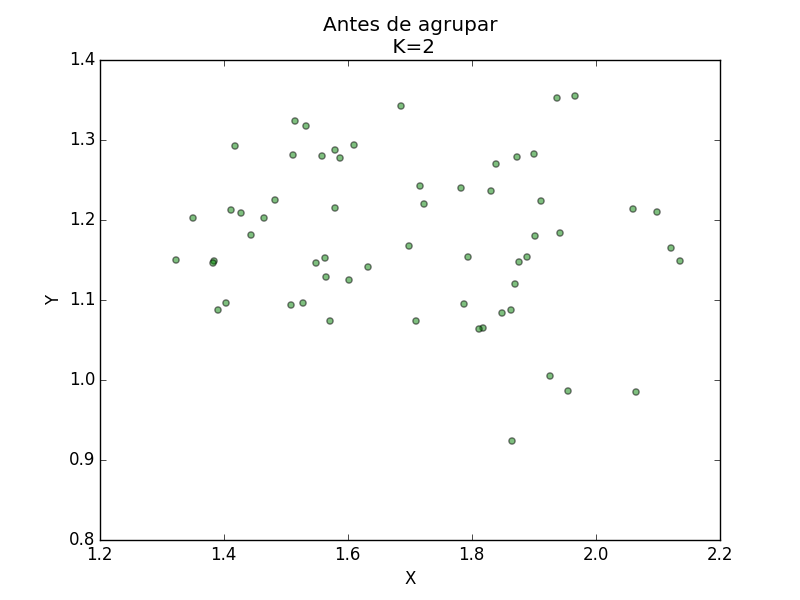
\includegraphics[width=0.4\textwidth]{antes_k2.png}
    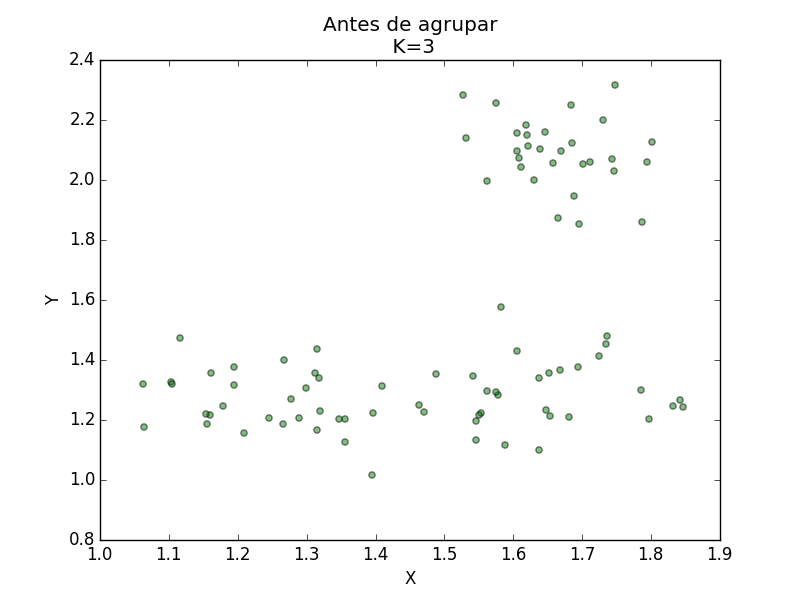
\includegraphics[width=0.4\textwidth]{antes_k3.png}
    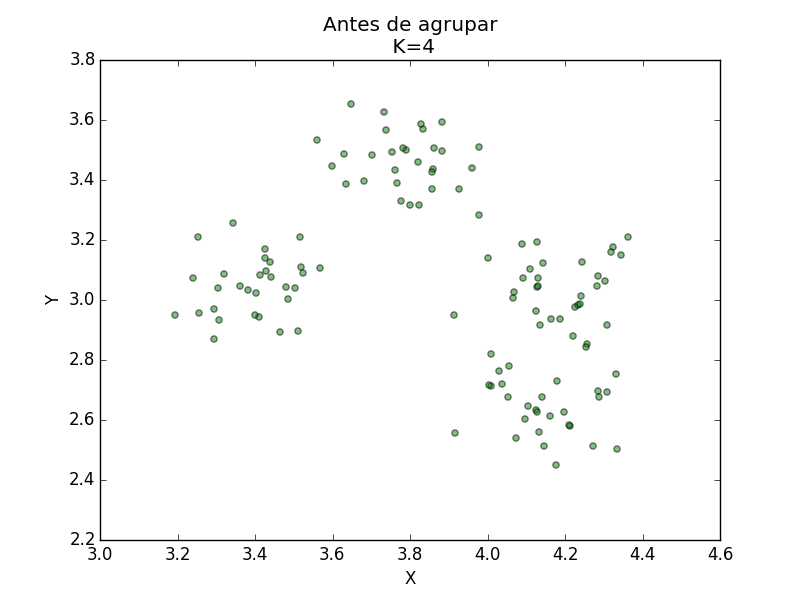
\includegraphics[width=0.4\textwidth]{antes_k4.png}
    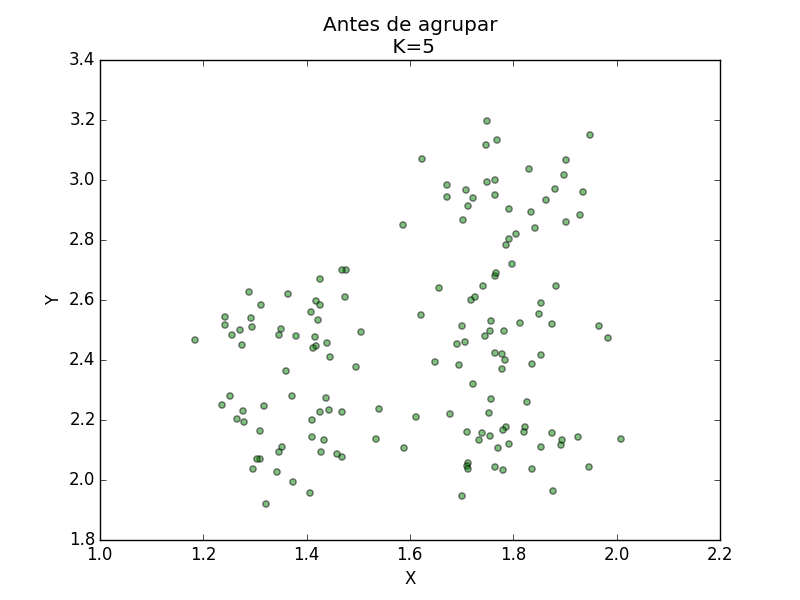
\includegraphics[width=0.4\textwidth]{antes_k5.png}
    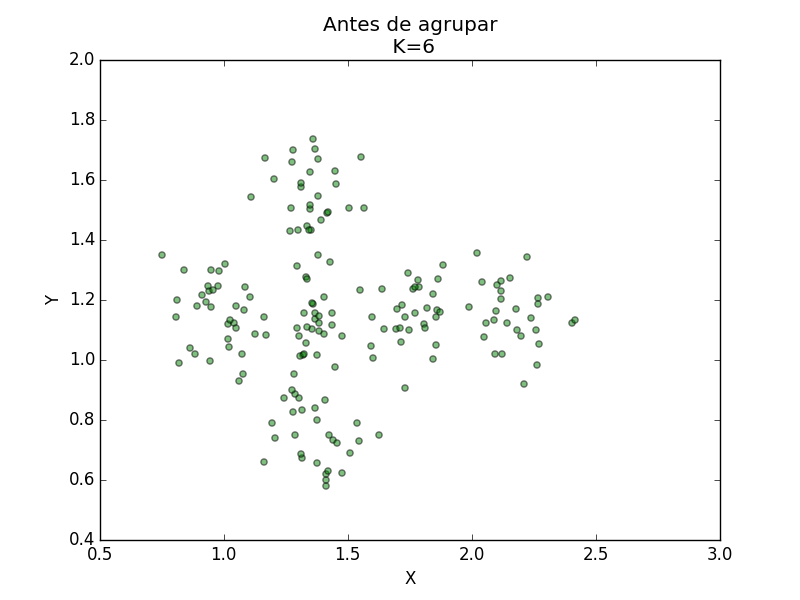
\includegraphics[width=0.4\textwidth]{antes_k6.png}
    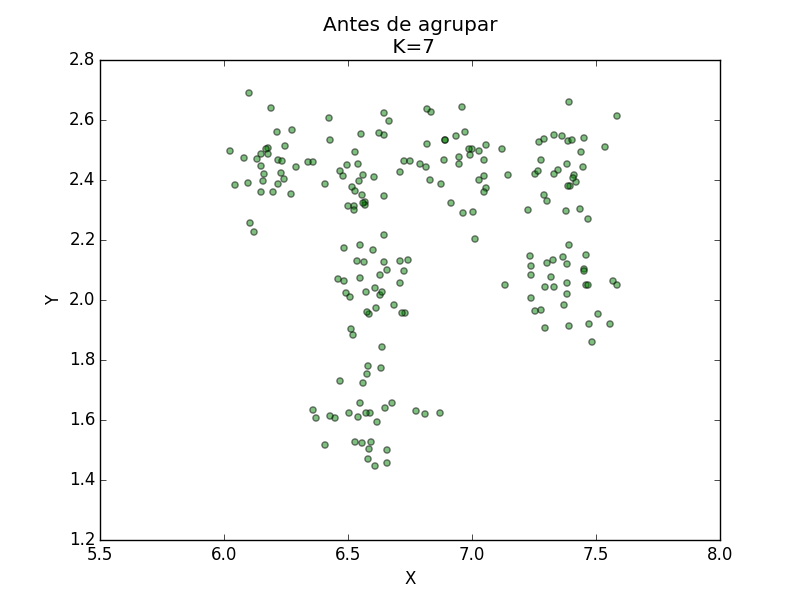
\includegraphics[width=0.4\textwidth]{antes_k7.png} 
    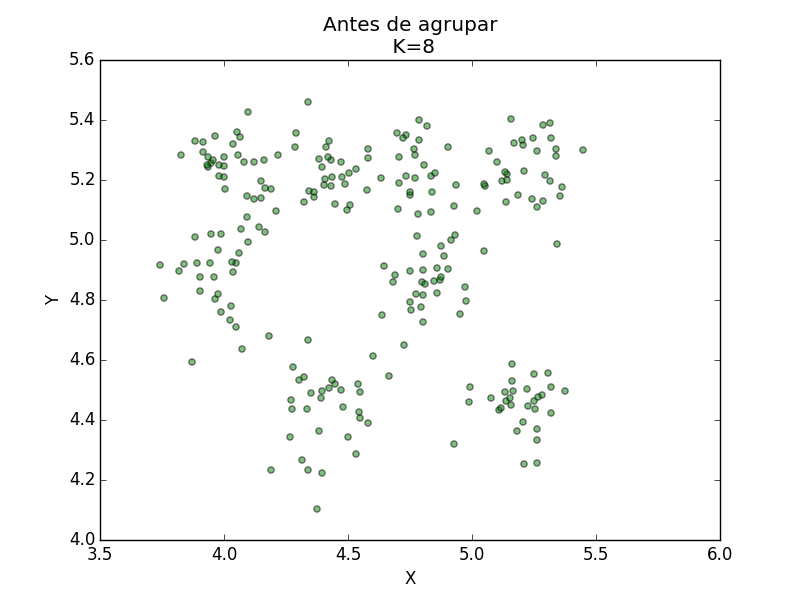
\includegraphics[width=0.4\textwidth]{antes_k8.png}    
    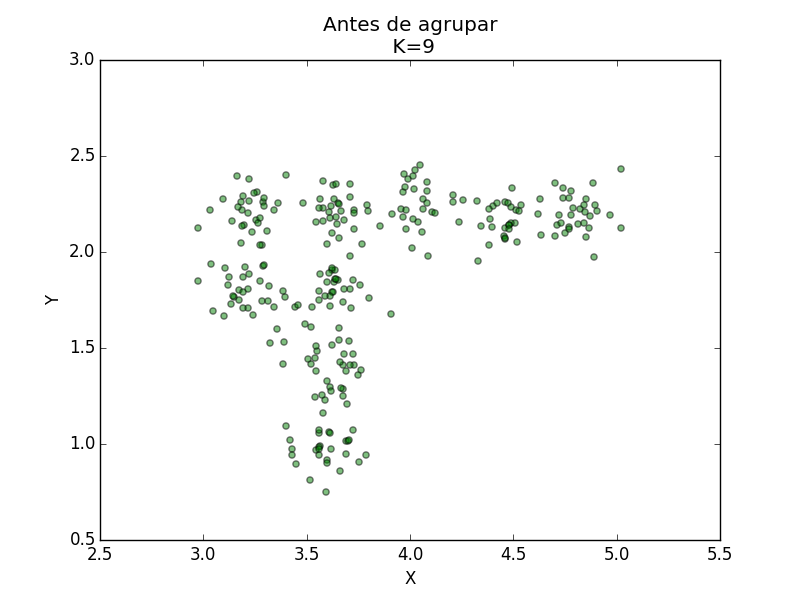
\includegraphics[width=0.4\textwidth]{antes_k9.png}
    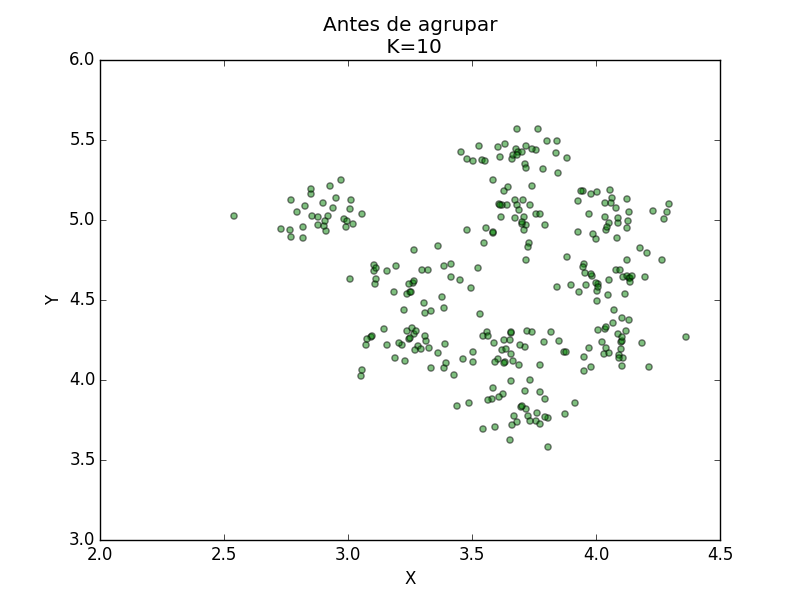
\includegraphics[width=0.4\textwidth]{antes_k10.png}          
\end{figure}
\end{landscape}

\begin{landscape}
\begin{figure}[!ht]
\label{erros}
  \caption{Evolução dos Somatórios de Erro Quadrático - SSE}
  \centering
    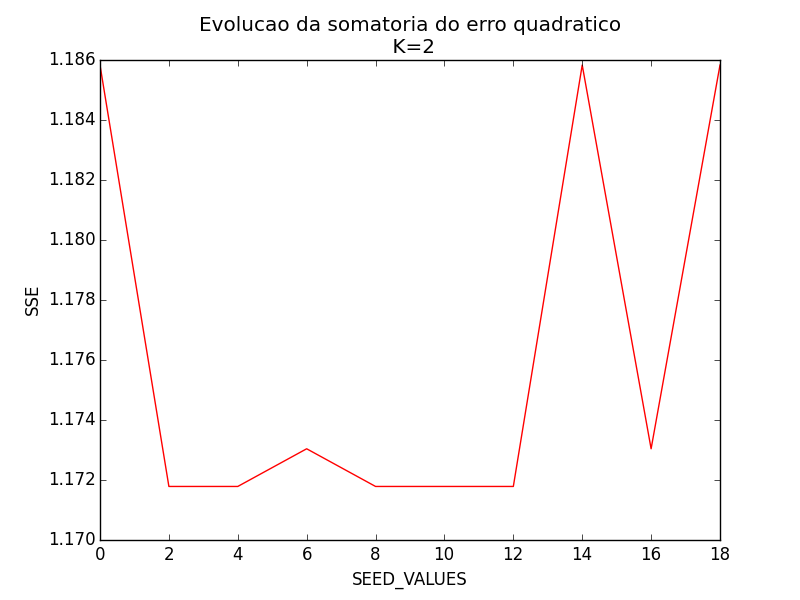
\includegraphics[width=0.4\textwidth]{erro_k2.png}
    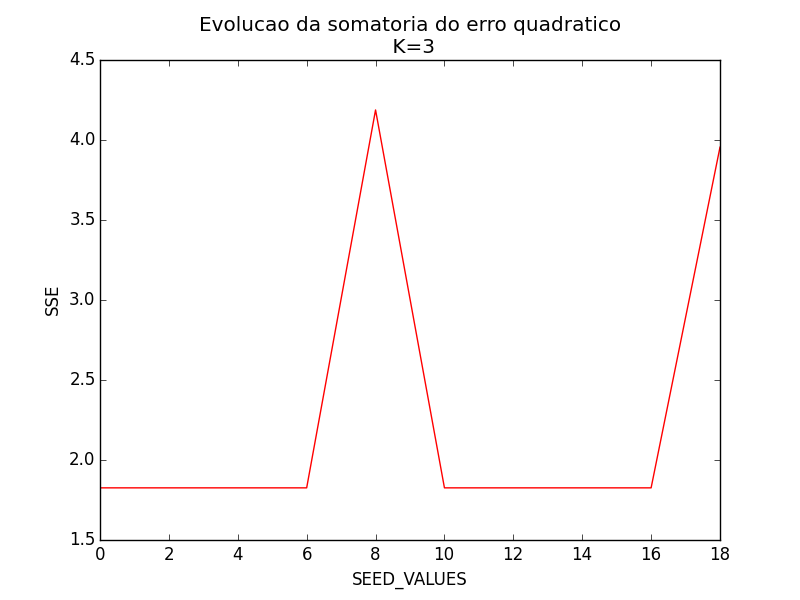
\includegraphics[width=0.4\textwidth]{erro_k3.png}
    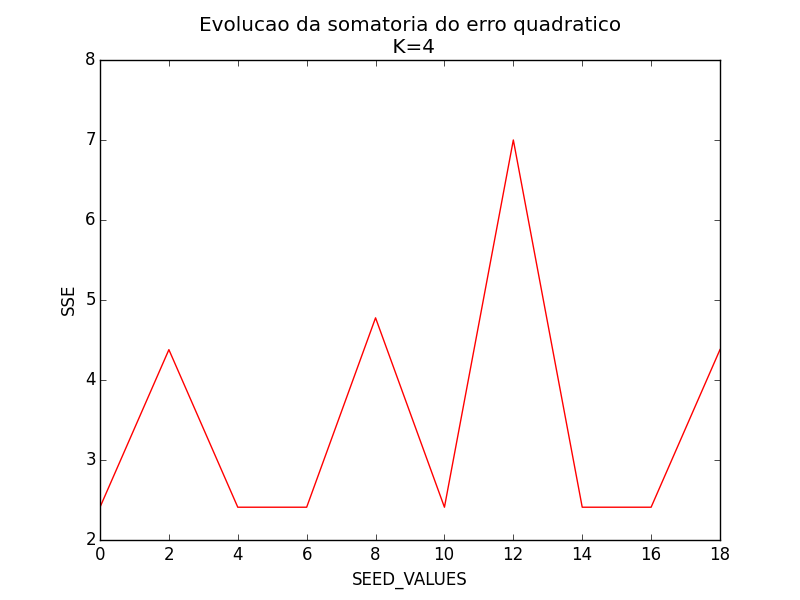
\includegraphics[width=0.4\textwidth]{erro_k4.png}
    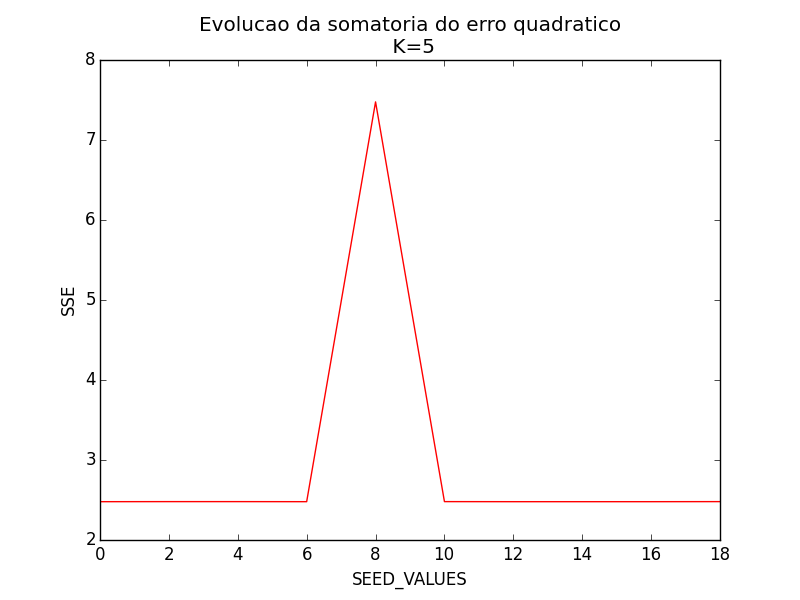
\includegraphics[width=0.4\textwidth]{erro_k5.png}
    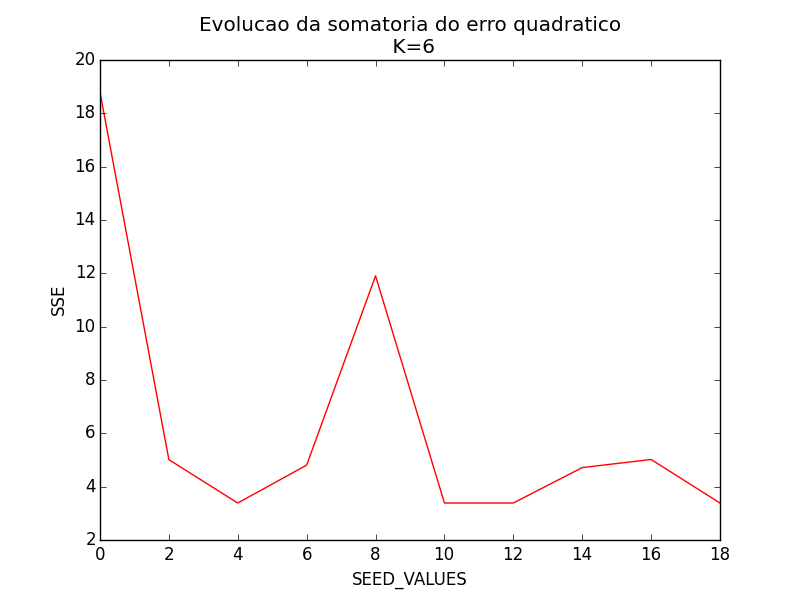
\includegraphics[width=0.4\textwidth]{erro_k6.png}
    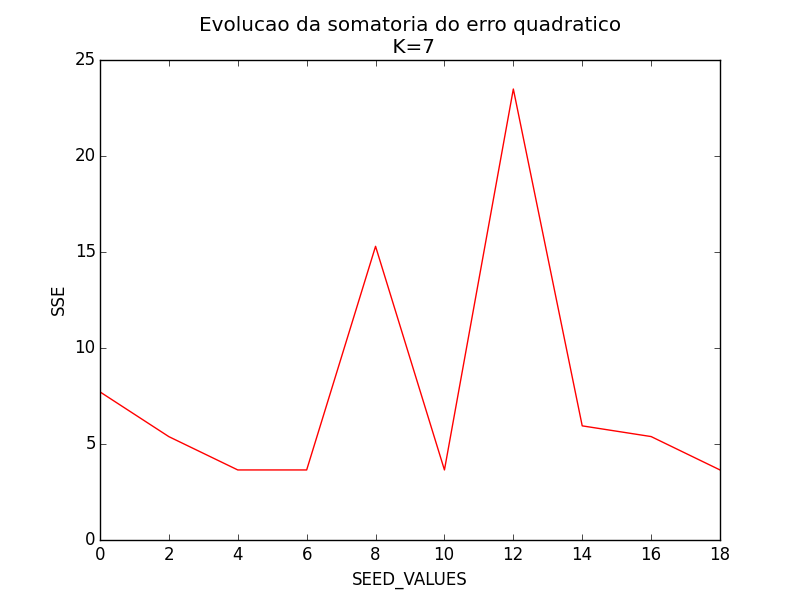
\includegraphics[width=0.4\textwidth]{erro_k7.png} 
    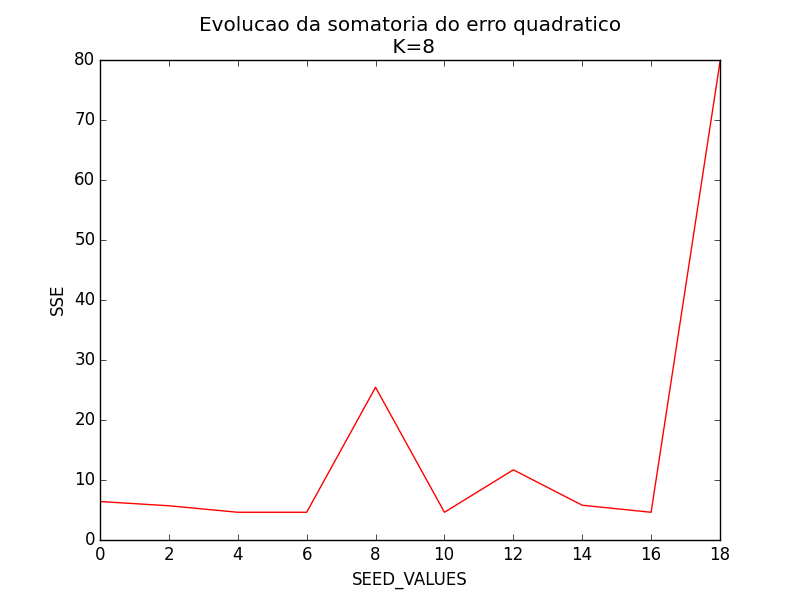
\includegraphics[width=0.4\textwidth]{erro_k8.png}    
    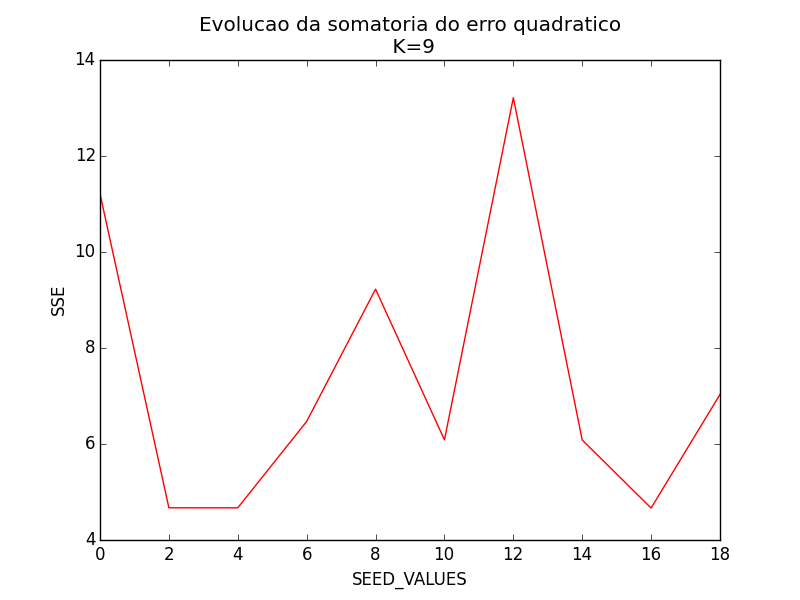
\includegraphics[width=0.4\textwidth]{erro_k9.png}
    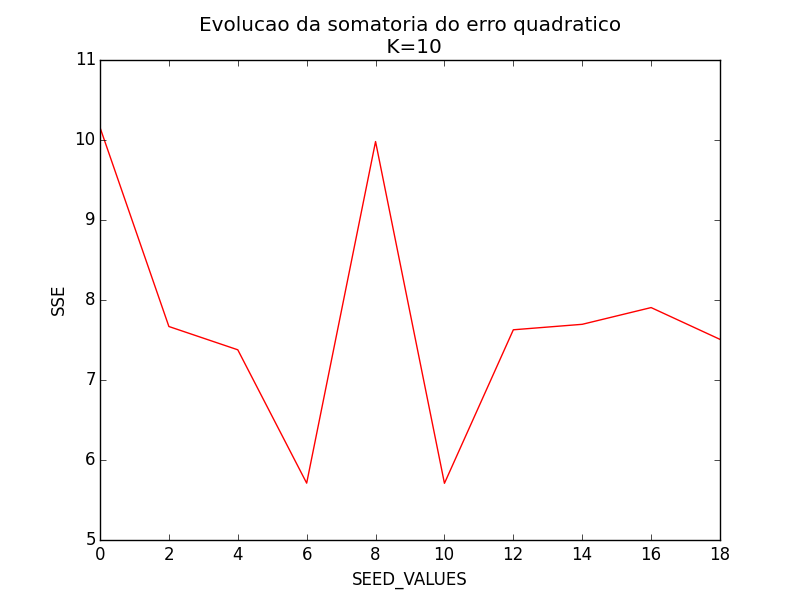
\includegraphics[width=0.4\textwidth]{erro_k10.png}
\end{figure}
\end{landscape}

\begin{landscape}
\begin{figure}[!ht]
\label{k=7}
  \caption{Exemplo de evolução do processo de agrupamento para k = 7}
  \centering
    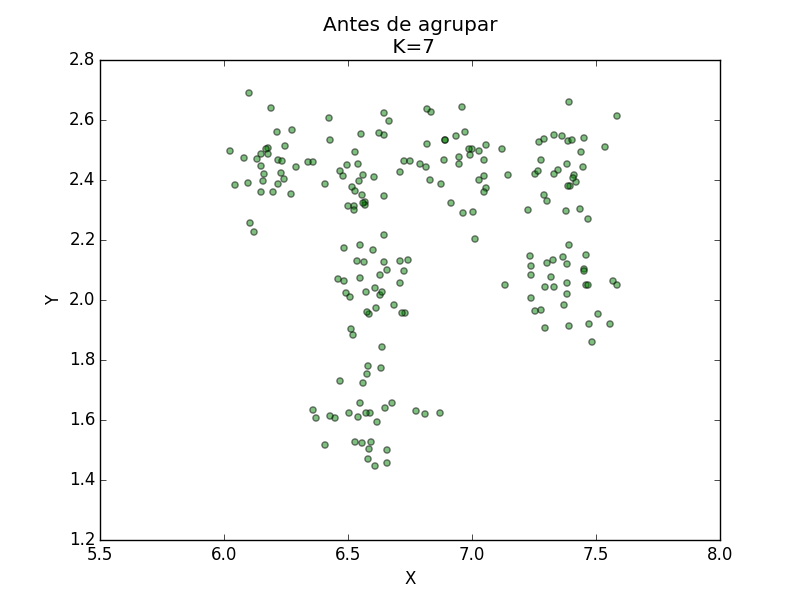
\includegraphics[width=0.42\textwidth]{antes_k7.png}
    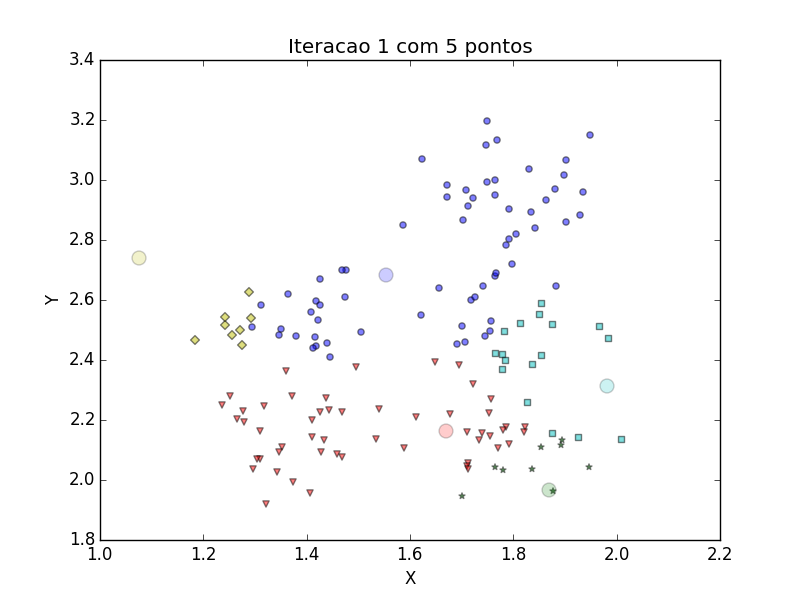
\includegraphics[width=0.42\textwidth]{depois_1.png}
    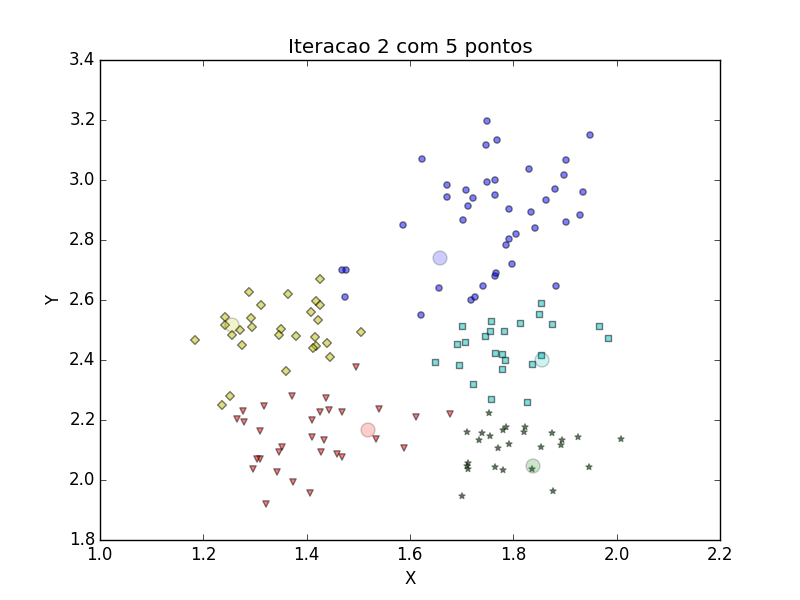
\includegraphics[width=0.42\textwidth]{depois_2.png}
    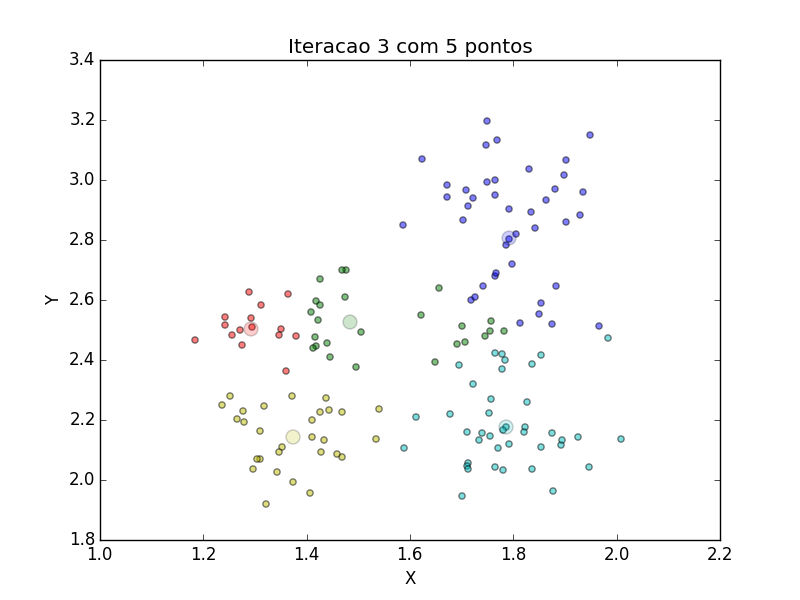
\includegraphics[width=0.42\textwidth]{depois_3.png}
    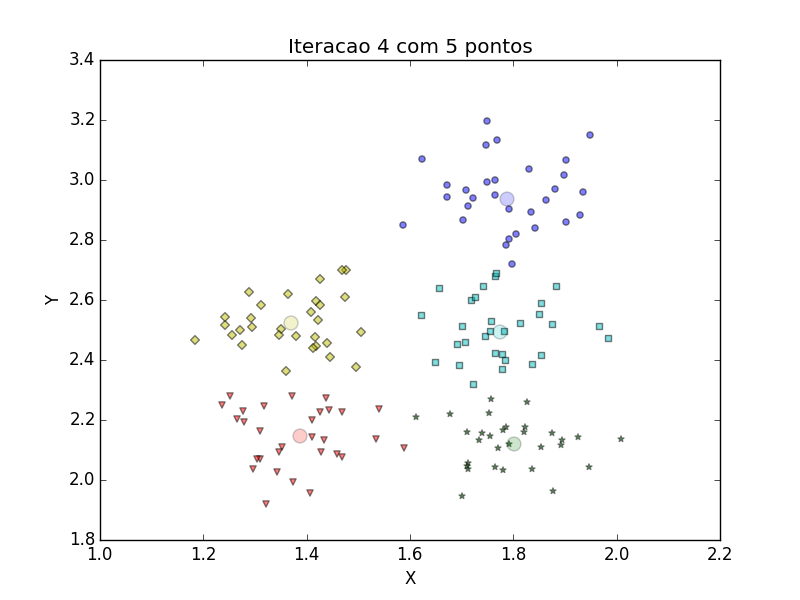
\includegraphics[width=0.42\textwidth]{depois_4.png}
    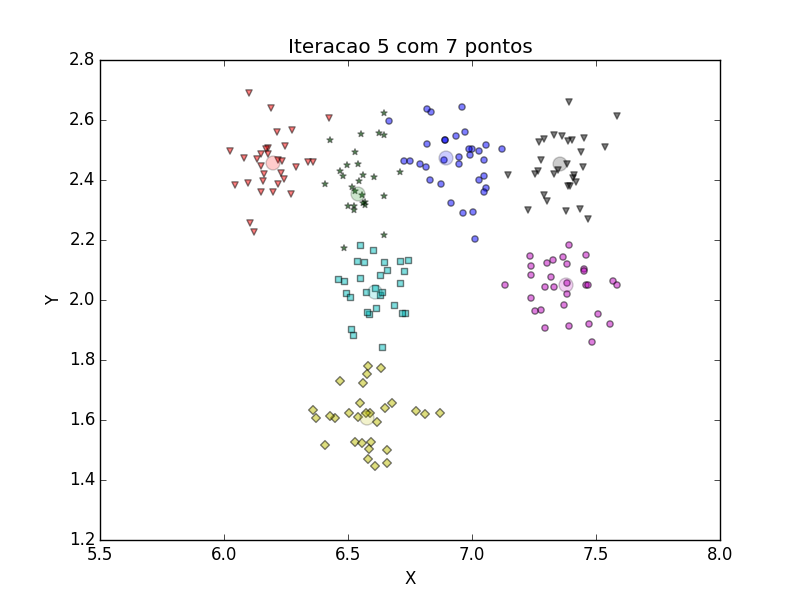
\includegraphics[width=0.42\textwidth]{depois_5.png} 
    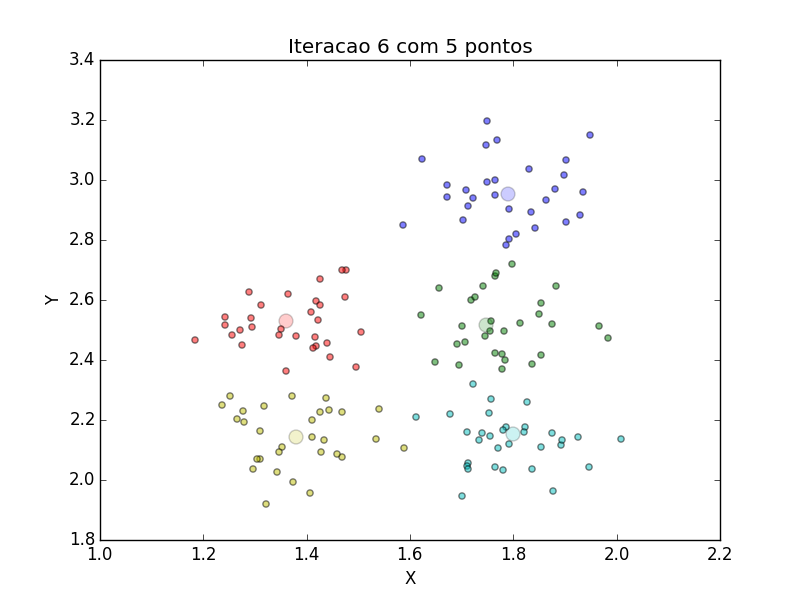
\includegraphics[width=0.42\textwidth]{depois_6.png}
    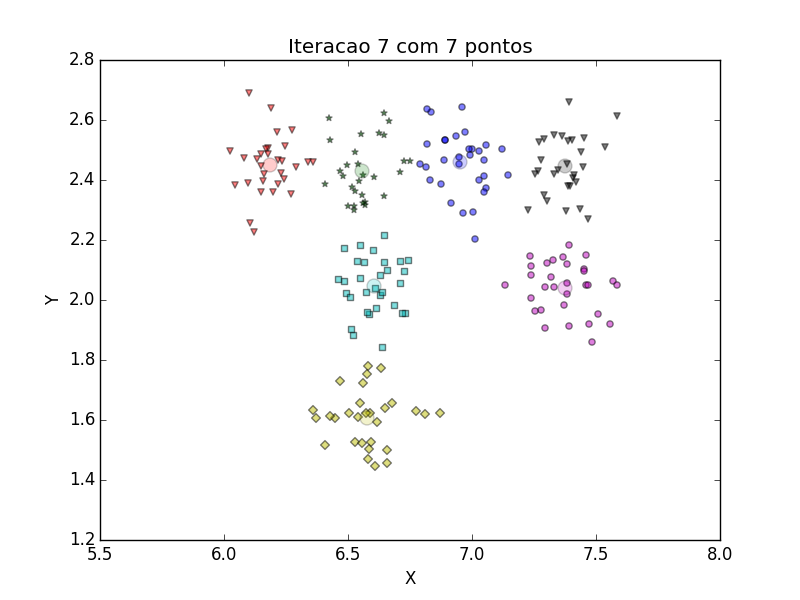
\includegraphics[width=0.42\textwidth]{depois_7.png} 
    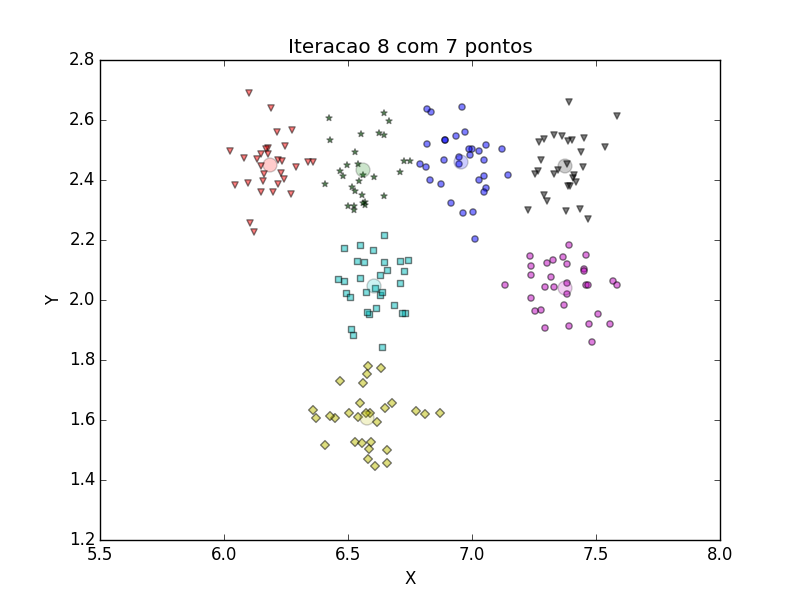
\includegraphics[width=0.42\textwidth]{depois_8.png}
\end{figure}
\end{landscape}

\section{Considerações Finais}
O algoritmo K-Médias é um algoritmo de agrupamento por particionamento. É eficiente, rápido e de razoável dificuldade de implementação. Seu ponto fraco consiste no fato de que os pontos aleatórios que se tornarão centros dos grupos não podem ser previstos ou controlados, necessitando uma séries de testes, com base na tentativa e erro, para se encontrar o melhor valor da semente da função de geração dos pontos aleatórios (\emph{seed}).

De posse de um bom conjunto de centros de grupos o algoritmo se mostra eficiente, tendo acurácia maior que 95\% para todos os casos de teste que nos foram passados e não precisando de muitas iterações para atingir a convergência.

No caso de escolha errada dos valores de \textit{seeds} pode-se incorrer em grupos vazios e no ``sumiço'' dos centros de grupo, prejudicando muito a eficiência do algoritmo.

Percebemos, com o uso do algoritmo, que o processo de agrupamento pode ser extremamente útil para a compreensão de grandes massas de dados e que a escolha de boas funções de distância e de geração randômica dos centros de grupo podem fazer a diferença entre o sucesso e o fracasso do trabalho de análise de dados.

\newpage
\bibliography{Trabalho_IA}

\end{document}